\documentclass[11pt, a4paper]{article}

\usepackage{graphicx}
\usepackage[a4paper,top=3cm,bottom=2cm,left=2cm,right=2cm,marginparwidth=1.75cm]{geometry}
\usepackage[english]{babel}
\usepackage[utf8x]{inputenc}
\usepackage{subfig}
\usepackage{float}
\usepackage{amsmath}
\usepackage{amssymb}
\usepackage{mhchem}
\usepackage{hyperref}
\usepackage{tikz}
\usepackage{cancel}

\graphicspath{ {./images} }
\newcommand*{\qed}{\hfill\ensuremath{\quad\square}}%
\newcommand*{\rad}{\ensuremath{\,\text{rad}}}
\newcommand*{\R}{\ensuremath{\mathbb{R}}}

\makeatletter
\renewcommand*\env@matrix[1][*\c@MaxMatrixCols c]{%
  \hskip -\arraycolsep
  \let\@ifnextchar\new@ifnextchar
  \array{#1}}
\makeatother

\newtheorem{theorem}{Theorem}
%------------------------------------------------
%Templates for images and figures
% \begin{figure}[h]
%   \centering
%   \subfloat[caption 1]{{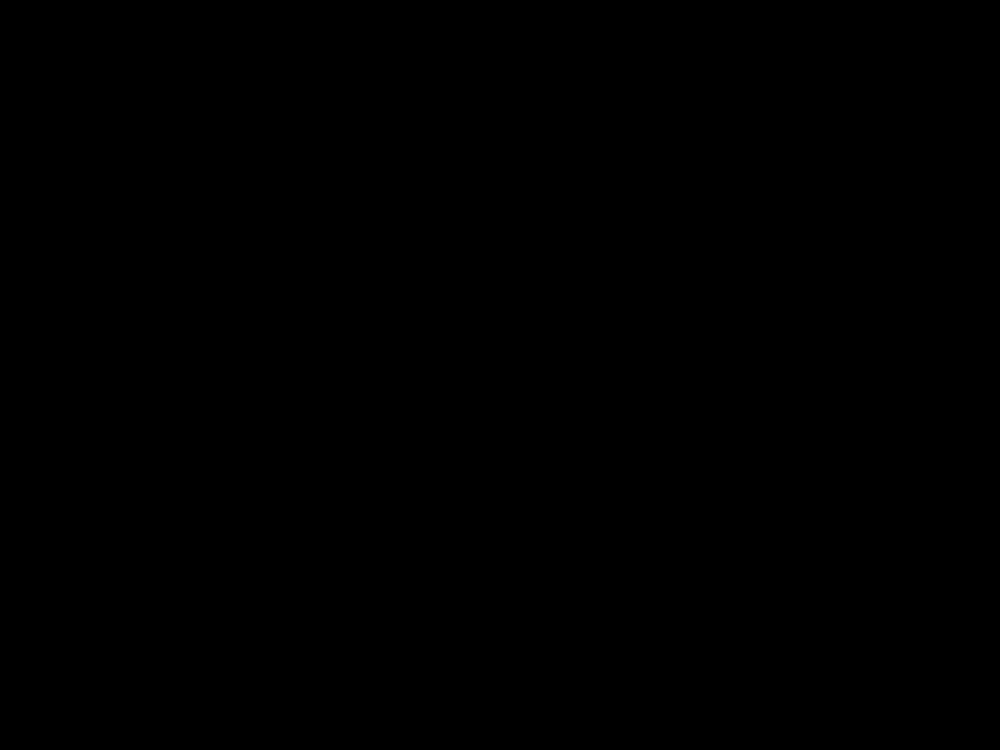
\includegraphics[width=30mm]{images/placeholder.png}}}%
%   \qquad
%   \subfloat[caption 2]{{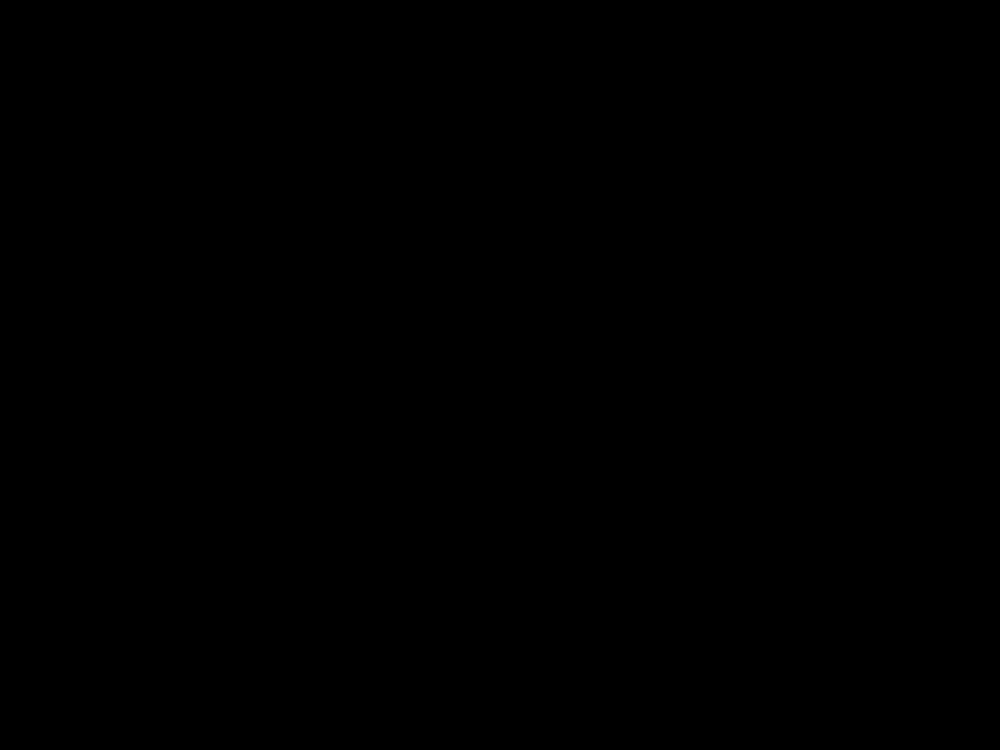
\includegraphics[width=30mm]{images/placeholder.png}}}%
%   \caption{Description}
% \end{figure}

% \begin{figure}[h]
%   \centerline{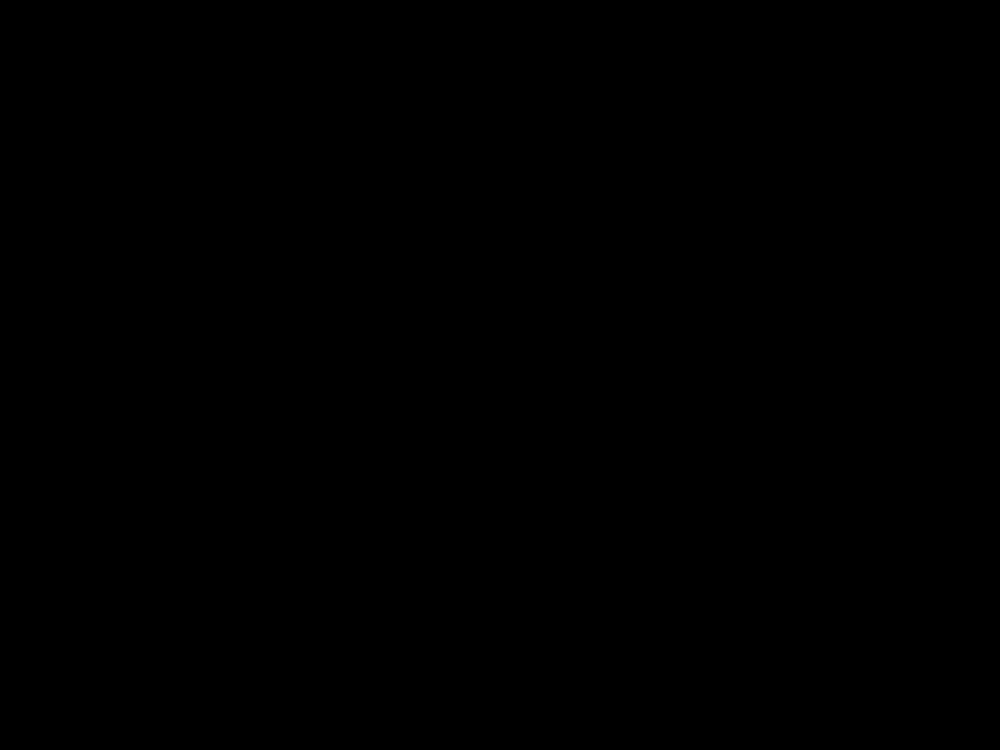
\includegraphics[width=50mm]{images/placeholder.png}}
%   \caption{Description}
% \end{figure}

%Template for a simple table 
%\begin{table}[h]
%   \caption{Description} %title of the table
%   \centering % centering table
%   \begin{tabular}{l rr} % creating three columns
%     \hline\hline %inserting double-line
%     & & \\ [0.5ex] % Insert half line vertical spacing
%     \hline % inserts single-line
%     & & \\ 
%     & & \\
%     & & \\
%     & & \\
%   \hline % inserts single-line
%   \end{tabular}
%   \label{tab:hresult}
% \end{table}
%-----------------------------------------------

\begin{document}
\setcounter{section}{8}
\setcounter{equation}{0}
\section{Thermofluids Lecture 9: The second Law of Thermodynamics (Part 1) (18/05/2020)}


\subsection{Introduction to the second law}
The second law of Thermodynamics tells us something about the direction of thermodynamics processes. Nature usually has a direction in which processes tend to happen spontaneously. For example: dropping a book from a height will turn pontential energy into kinetic energy. When the book hits the ground kinetic energy will turn into sound and heat on impact. However, simply boiling the book and yelling at it for a bit will \underline{not} make it fall back up. In other words it's a one way trip. Whenever processes do happen spontaneously there is an imbalance between begin- and end-state of the system. There is a non-equilibrium. Furthermore the second law limits the amount of work that can be obtained from any random power cycle. The second law of thermodynamics is formally given as: \newline
\textit{the total entropy of an isolated system can never decrease over time, and is constant if and only if all processes are reversible. Isolated systems spontaneously evolve towards thermodynamic equilibrium, the state with maximum entropy.}


\subsection{Reversibility of processes}
A system which can be considered reversible is any systems which statisfies all of the following properties:
\begin{itemize}
  \item The system and it's surroundings can at all times return to their original state
  \item If the process is reversed, then it's forward path and backward path will be indentical
\end{itemize}
Some interesting things of note are the following: Perfectly reversible systems can \underline{never} be reached in practice. The surroundings will always be altered in some way. Furthermore a perfectly reversible system cannot deviate from thermal equilibrium. This would make it infinitly slow. These properties also imply that an irreversible process can never spontaneously return to it's initial state.\\
\\
There may be several reasons as to why a process may not be reversible. Some examples are:
\begin{itemize}
  \item All forms of friction
  \item Non-utilized heat transfer through difference in temperature
  \item Non-utilized expansion of fluid to a lower pressure
  \item Mixing of substances
  \item Electrical current flowing through a resistance
\end{itemize}
Irreversibilities are the parts of a process which reduce work that would theoretically be obtained if the process were reversible. Effectifly they are a loss in potential work that the system could do. Sometimes referred to as "lost" work.


\subsection{Internally reversible processes and thermal efficiency}
For all states of an interanlly reversible process that a closed system undergoes, all intensive state properties remain uniform in each of the phases present. This implies that the intensive properties do not change in space. A difference in intensive properties should lead to driving forces, whereas reversibility requires that no spontaneous process can take place.\\
We can use the idea that intensive properties do not change for these type of systems to describe thermal efficiency of a power cycle:
\begin{equation}
  \eta_{th} = \frac{\Delta^{cycle}W}{Q_{in}^H}
\end{equation}
We know that for internally reversible processes $\Delta^{cycle}W = Q_{in}^H - Q_{out}^H$. Subsituting this into the previous equation leaves us with:
\begin{equation}
  \eta_{th} = 1 - \frac{Q_{out}^H}{Q_{in}^H} < 1
\end{equation}
Because $Q_C^{cycle} > 0$ we can know for sure that $\eta_{th} < 0$, which makes alot of sense. A process can never output more work then what was initially put into it. Even a reversible (read idealized) power cycle process has a thermal efficiency lower then $1$, since heat can \underline{never} be fully converted to work.


\subsection{Results of the second law}
The second law has many implications. The first of which is, as discussed before, that $\eta_{th} < 1$ for any process or power cycle. Furthermore all reversible Carnot-like\footnote{Carnot-like means all external heat transfer is realized isothermally with 2 thermal reservoirs.} (more on that later) power cycles operating between the same temperature of 2 thermal reservoirs have the same thermal efficiency $\eta_{rev}$. This implies that $\eta_{th}$ for a Carnot-like power cycle is independent of working fluid and independent of the processes making up the cycle. An irreversible (read real) power cycle has a lower efficiency still, since it accounts for Irreversibilities. Thus we are left with the following inequality:
\begin{equation}
  \eta_{real} < \eta_{rev} < 1
\end{equation}


\subsection{The Carnot power cycle process for ideal gas}
The Carnot cycle generally refers to a $4$ step idealized power cycle. It's a perfectly reversible process. An heat engine using a Carnot-cycle is a "perfect" heat engine. It's usefull for modelling maximum achievable efficiency of power cycles. The steps for a Carnot cycle are:
\begin{enumerate}
  \item process $1 \to 2$: Reversible isothermal expansion
  \item process $2 \to 3$: Reversible adiabatic expansion
  \item process $3 \to 4$: Reversible isothermal compression
  \item process $4 \to 1$: Reversible adiabatic compression
\end{enumerate}
\begin{figure}[h]
  \centerline{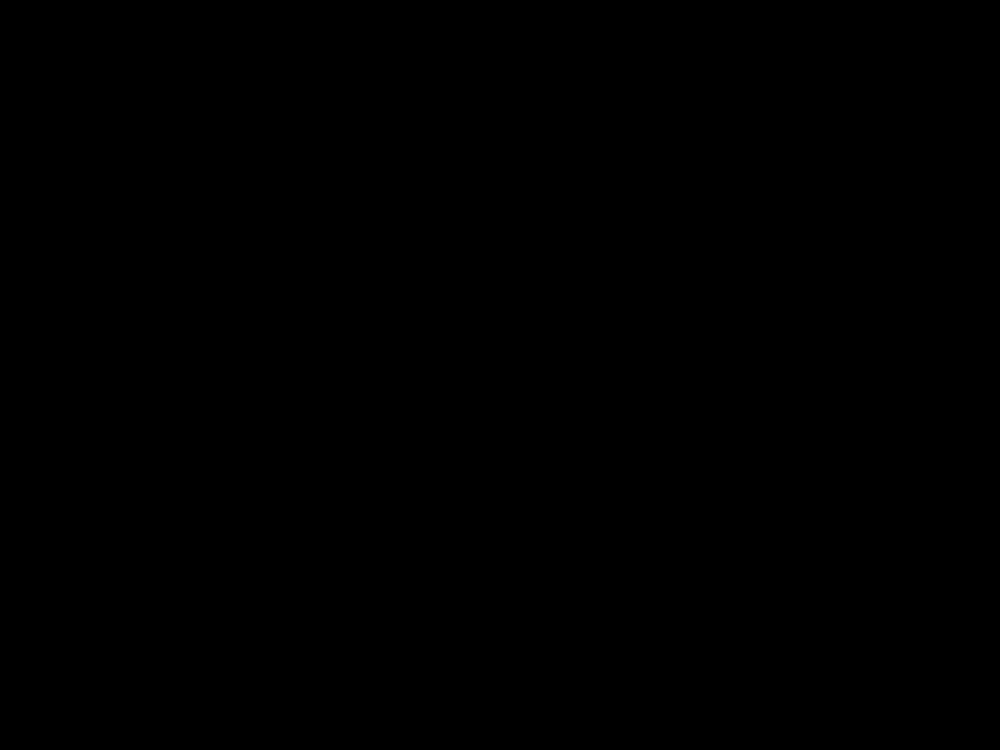
\includegraphics[width=80mm]{images/placeholder.png}}
  \caption{The carnot cycle process for which the derrivation will be made}
  \label{fig:Carnot_cycle}
\end{figure}
Consider the Carnot-cycle given in figure \ref{fig:Carnot_cycle}. $T_H$ and $T_C$ are isotherms along which the temperature is constant.\\
\\ 
\underline{Process $1 \to 2$:}
\begin{align}
  W_{12} = \int_1^2 p\,dV &= \int_1^2 \frac{mRT_C}{V}\,dV\\
                          &= mRT_C \ln \left( \frac{V_2}{V_1} \right)
\end{align}
We know the process is internally reversible, thus $\Delta U =0$:
\begin{gather}
  \Delta Q_{12} = \cancelto{0}{\Delta U_{12}} + W_{12}\\
  W_{12} = \Delta Q_{12} = mRT_C \ln \left( \frac{V_2}{V_1} \right)
\end{gather}\\
\\
\underline{Process $2 \to 3$:}
\begin{equation}
  p_2V_2^\kappa = p_3V_3^\kappa \Rightarrow p = p_2 \left( \frac{V_2}{V} \right)^\kappa
\end{equation}
Using this equation we can compute the work as follows:
\begin{align}
  W_{23} = \int_2^3 p\,dV &= p_2V_2^\kappa \int_2^3 V^{-\kappa}\,dV\\
                          &= \left.\frac{p_2V_2^\kappa}{1 - \kappa}(1-\kappa)\right|_2^3\\
                          &= \frac{p_2V_2^\kappa}{1-\kappa}(V_3^{1-\kappa} - V_2^{1-\kappa})\\
                          &= \frac{mR(T_H - T_C)}{\kappa - 1}
\end{align}\\
\\
\underline{Process $3 \to 4$:}
\begin{align}
  W_{34} = \int_3^4 p\,dV &= \int_3^4 \frac{mRT_H}{V}\,dV\\
                          &= mRT_H \ln \left( \frac{V_4}{V_3} \right)
\end{align}
We again know that $\Delta U = 0$, which leads to the following:
\begin{gather}
  \Delta Q_{34} = \cancelto{0}{\Delta U_{34}} + W_{34}\\
  W_{34} = \Delta Q_{34} = mRT_H \ln \left( \frac{V_4}{V_3} \right)
\end{gather}\\
\\
\underline{Process $4 \to 1$:}
Note that $T_1 = T_C$ and that $T_4 = T_H$.
\begin{align}
  W_{41} = \int_4^1 p\,dV &= \frac{-mR(T_C - T_H)}{\kappa - 1}\\
                          &= \frac{mR(T_H - T_C}{\kappa - 1}
\end{align}\\
We now have all the individual components which add up to the total work of the cycle. The thermal efficiency of a cycle is described by:
\begin{equation}
  \eta_{cycle} = \frac{W_{cycle}}{Q_H} \quad \text{where} \quad W_{cycle} = \Sigma W
\end{equation}
This ends us up with the following:
\begin{equation}
  \eta_{cycle} = \frac{W_{12} + W_{23} + W_{34} + W_{41}}{Q_{34}}
\end{equation}
Walking through the algebra\footnote{I can't be fucked to write it down here cause it's a lengthy one} then gives the following relation:
\begin{equation}
  \eta_{cycle} = \frac{T_H - T_C}{T_H} = 1 - \frac{T_C}{T_H}
\end{equation}

\subsection{Introducing entropy}
Entropy is a bit of an abstract property that is difficult to conceptualize. It can be thought of as the amount of disorder of a given system. In general without an external source disorder only increase. For example atoms would like to diffuse as much as possible across a space as this is the most chaotic state. This means that for a closed system entropy will always be greater then (or equal to in some idealized cases) to $0$. The universe can be considered an isolated system, thus the total entropy is always increasing. Marching us closer and closer to the inevitable end of time by heat death of the universe! Note that entropy is not a conserved quantity. There is no "conservation of entropy" law.\\
Consider the thermal efficiency of a given Carnot cycle:
\begin{equation*}
  \eta_{cycle} = 1 - \frac{Q_C}{Q_H} = 1 - \frac{T_C}{T_H}
\end{equation*}
This implies the following:
\begin{equation*}
  \frac{Q_C}{Q_H} = \frac{T_C}{T_H} \Rightarrow \frac{Q_H}{T_H} - \frac{Q_C}{T_C} = 0
\end{equation*}
This extends to any random Carnot cycle of $n$ steps:
\begin{equation*}
  \frac{Q_{12}}{T_{12}} + \frac{Q_{23}}{T_{23}} + \cdots + \frac{Q_{n1}}{T_{n1}} = 0
\end{equation*}
Since a Carnot cycle is perfectly reversible all the internal energies should equal $0$, thus:
\begin{equation*}
  \Delta U_{12} + \Delta U_{23} + \cdots + \Delta U_{n1} = 0
\end{equation*}
We know that this total sum of variables equaling $0$ only happens to state variables. Yet $Q$ is not a state variable. Thus Clausius defined a new state variable: Entropy, denoted as $S$.
\begin{equation}
  \Delta S_{12} + \Delta S_{23} + \cdots + \Delta S_{n1} = 0
\end{equation}
The variable $S$, entropy, is used to denote the direction of processes. In diffential form entropy for an internally reversible process is given as:
\begin{equation}
  \left. \frac{\delta Q}{T} \right|_{int,rev} = dS
\end{equation}
For internally reversible processes we can write this as a cyclic integral (read an integral along the entire cycle) as follows:
\begin{equation}
  \oint \frac{\delta Q}{T} = \oint dS = 0
\end{equation}


\subsection{The Clausius inequality}
The Clausius inequality is given as:
\begin{equation}
  \oint \frac{\delta Q}{T} \leq 0
\end{equation}
This expression basicly states that a system undergoing a cycle returns to it's original state.\\
Consider a cycle with 2 processes. The process $1 \to 2$ which is either reversible or irreversible and process $2 \to 1$ which is internally reversible. Then applying the Clausius inequality we get:
\begin{equation}
  \oint \frac{\delta Q}{T} = \int_1^2 \frac{\delta Q}{T} + \int_2^1 \left. \frac{\delta Q}{T} \right|_{int,rev} \leq 0
\end{equation}
Since $\left. \frac{\delta Q}{T}\right|_{int,rev} = dS$:
\begin{equation}
  \int_1^2 \frac{\delta Q}{T} + \int_2^1 dS = \int_1^2 \frac{\delta Q}{T} + S_1 - S_2 \leq 0
\end{equation}
Which rearranges to:
\begin{equation}
  S_2 - S_1 \geq \int_1^2 \frac{\delta Q}{T}
\end{equation}
The term $\int_1^2 \delta Q/T$ represents the entropy transfer by heat. We know that $S_2 - S_1 = \Delta S$. For a reversible system this becomes equal to entropy transfer. The inequality sign however still implies that some entropy is generated (might still be equal to 0 for idealized processes):
\begin{equation}
  \Delta S_{sys} = S_2 - S_1 = \int_1^2 \frac{\delta Q}{T} + S_{gen}
\end{equation}
$S_{gen}$ might sometimes also be noted by the letter $\sigma$. Note that this increase in entropy principle does not actually imply entropy of a system cannot be negative. Water freezing for example goes from a more chaotic state (liquid) to a more ordered state (solid). This implies a decrease in entropy. This may very well be valid as long as the entropy generated is equal to $0$ and the sum of the entropy of the system and the surroundings is positive.
\begin{equation}
  S_{gen} = \Delta S_{total} = \Delta S_{sys} + \Delta S_{sur} \geq 0
\end{equation}
We can say the following about entropy generated:
\begin{equation}
  S_{gen}
  \begin{cases}
    > 0, \text{irreversible process}\\
    = 0, \text{reversible process}\\
    < 0, \text{impossible process}
  \end{cases}
\end{equation}

\end{document}